\section{ObjectLogger Klassenreferenz}
\label{classObjectLogger}\index{ObjectLogger@{ObjectLogger}}
Klassendiagramm für ObjectLogger::\begin{figure}[H]
\begin{center}
\leavevmode
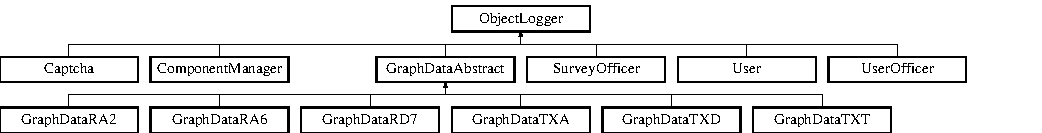
\includegraphics[height=1.79104cm]{classObjectLogger}
\end{center}
\end{figure}
\subsection*{Öffentliche Methoden}
\begin{CompactItemize}
\item 
{\bf ObjectLogger} ()
\item 
{\bf setRequiredDefinitions} (\$array)
\item 
{\bf \_\-validateRequiredDefinitions} ()
\item 
{\bf \_\-resetErrors} ()
\item 
{\bf hasErrors} ()
\item 
{\bf \_\-addError} (\$error, \$valueName=null)
\item 
{\bf getErrors} ()
\item 
{\bf getLastError} ()
\end{CompactItemize}
\subsection*{Öffentliche Attribute}
\begin{CompactItemize}
\item 
{\bf \$\_\-errorArray}
\item 
{\bf \$\_\-requiredDefinitionsArr}
\end{CompactItemize}


\subsection{Ausführliche Beschreibung}


Definiert in Zeile 7 der Datei class.ObjectLogger.php.

\subsection{Dokumentation der Elementfunktionen}
\index{ObjectLogger@{ObjectLogger}!ObjectLogger@{ObjectLogger}}
\index{ObjectLogger@{ObjectLogger}!ObjectLogger@{ObjectLogger}}
\subsubsection{\setlength{\rightskip}{0pt plus 5cm}ObjectLogger.ObjectLogger ()}\label{classObjectLogger_51e1001bd0063f27980e825ff7fea920}




Definiert in Zeile 30 der Datei class.ObjectLogger.php.\index{ObjectLogger@{ObjectLogger}!setRequiredDefinitions@{setRequiredDefinitions}}
\index{setRequiredDefinitions@{setRequiredDefinitions}!ObjectLogger@{ObjectLogger}}
\subsubsection{\setlength{\rightskip}{0pt plus 5cm}ObjectLogger.setRequiredDefinitions (\$ {\em array})}\label{classObjectLogger_32e3e4869d931bf1da2e2ce9e6a0ec4b}


set array of required definitions

\begin{Desc}
\item[Parameter:]
\begin{description}
\item[{\em array}]\$array \end{description}
\end{Desc}


Definiert in Zeile 39 der Datei class.ObjectLogger.php.

Wird benutzt von Captcha.Captcha() und UserOfficer.UserOfficer().\index{ObjectLogger@{ObjectLogger}!\_\-validateRequiredDefinitions@{\_\-validateRequiredDefinitions}}
\index{\_\-validateRequiredDefinitions@{\_\-validateRequiredDefinitions}!ObjectLogger@{ObjectLogger}}
\subsubsection{\setlength{\rightskip}{0pt plus 5cm}ObjectLogger.\_\-validateRequiredDefinitions ()}\label{classObjectLogger_8db680194e6024d5a7e2db03d8d840e3}


Validate required definitions. Set it before with \$this-$>$setRequiredDefinitions(array('DENITION1','DENITION2'));

\begin{Desc}
\item[Rückgabe:]bool \end{Desc}


Definiert in Zeile 48 der Datei class.ObjectLogger.php.

Wird benutzt von Captcha.\_\-initialize().\index{ObjectLogger@{ObjectLogger}!\_\-resetErrors@{\_\-resetErrors}}
\index{\_\-resetErrors@{\_\-resetErrors}!ObjectLogger@{ObjectLogger}}
\subsubsection{\setlength{\rightskip}{0pt plus 5cm}ObjectLogger.\_\-resetErrors ()}\label{classObjectLogger_3b306238378bb21cf09333e0ce691c0b}


Reset error stack  private 

Definiert in Zeile 64 der Datei class.ObjectLogger.php.

Wird benutzt von getErrors(), getLastError() und ComponentManager.loadComponents().\index{ObjectLogger@{ObjectLogger}!hasErrors@{hasErrors}}
\index{hasErrors@{hasErrors}!ObjectLogger@{ObjectLogger}}
\subsubsection{\setlength{\rightskip}{0pt plus 5cm}ObjectLogger.hasErrors ()}\label{classObjectLogger_c8a2fbf95ac1aa972132dec5e4d5ee79}


Check if function has errors  public \begin{Desc}
\item[Rückgabe:]bool \end{Desc}


Definiert in Zeile 74 der Datei class.ObjectLogger.php.\index{ObjectLogger@{ObjectLogger}!\_\-addError@{\_\-addError}}
\index{\_\-addError@{\_\-addError}!ObjectLogger@{ObjectLogger}}
\subsubsection{\setlength{\rightskip}{0pt plus 5cm}ObjectLogger.\_\-addError (\$ {\em error}, \$ {\em valueName} = {\tt null})}\label{classObjectLogger_80da39713b2275b8a78d4d9a3f43b34f}


adds error to error stack

private \begin{Desc}
\item[Parameter:]
\begin{description}
\item[{\em string}]\$error \item[{\em string}]\$valueName \end{description}
\end{Desc}


Definiert in Zeile 89 der Datei class.ObjectLogger.php.

Wird benutzt von GraphDataAbstract.\_\-loadGraphData(), SurveyOfficer.createSurvey(), SurveyOfficer.getSurveyConstants(), ComponentManager.loadComponents(), User.setEmail(), User.setPassword() und SurveyOfficer.updateSurvey().\index{ObjectLogger@{ObjectLogger}!getErrors@{getErrors}}
\index{getErrors@{getErrors}!ObjectLogger@{ObjectLogger}}
\subsubsection{\setlength{\rightskip}{0pt plus 5cm}ObjectLogger.getErrors ()}\label{classObjectLogger_972ed527bf7f3ff3a7cf0a00b2eb8f59}


returns array of errors

public \begin{Desc}
\item[Rückgabe:]array \end{Desc}


Definiert in Zeile 103 der Datei class.ObjectLogger.php.

Benutzt \_\-resetErrors().\index{ObjectLogger@{ObjectLogger}!getLastError@{getLastError}}
\index{getLastError@{getLastError}!ObjectLogger@{ObjectLogger}}
\subsubsection{\setlength{\rightskip}{0pt plus 5cm}ObjectLogger.getLastError ()}\label{classObjectLogger_4dff6e98f5955e509a4db5ed9f01e075}


Gives lastError as text if accuiried

public \begin{Desc}
\item[Autor:]Mischa Kupriyanov, $<${\tt m@kupriyanov.com}$>$ \end{Desc}
\begin{Desc}
\item[Rückgabe:]string \end{Desc}


Definiert in Zeile 116 der Datei class.ObjectLogger.php.

Benutzt \_\-resetErrors().

\subsection{Dokumentation der Datenelemente}
\index{ObjectLogger@{ObjectLogger}!\$\_\-errorArray@{\$\_\-errorArray}}
\index{\$\_\-errorArray@{\$\_\-errorArray}!ObjectLogger@{ObjectLogger}}
\subsubsection{\setlength{\rightskip}{0pt plus 5cm}ObjectLogger.\$\_\-errorArray}\label{classObjectLogger_d5bd26e05691edf51c66e586884ec434}




Definiert in Zeile 21 der Datei class.ObjectLogger.php.\index{ObjectLogger@{ObjectLogger}!\$\_\-requiredDefinitionsArr@{\$\_\-requiredDefinitionsArr}}
\index{\$\_\-requiredDefinitionsArr@{\$\_\-requiredDefinitionsArr}!ObjectLogger@{ObjectLogger}}
\subsubsection{\setlength{\rightskip}{0pt plus 5cm}ObjectLogger.\$\_\-requiredDefinitionsArr}\label{classObjectLogger_df651a233ca51d5632226904f6fd83b0}




Definiert in Zeile 28 der Datei class.ObjectLogger.php.

Die Dokumentation für diese Klasse wurde erzeugt aufgrund der Datei:\begin{CompactItemize}
\item 
{\bf class.ObjectLogger.php}\end{CompactItemize}
